% !TeX spellcheck = en_US
\documentclass[12pt, a4paper, titlepage]{book}
%\usepackage[a4paper, margin=3cm]{geometry}

%
\usepackage[utf8]{inputenc}			% utf-8, bitches
\usepackage[T1]{fontenc}			% das Trennen der Umlaute
\usepackage[english]{babel}			% word wrapping

\usepackage{parskip}				% makes paragraph spacing nicer
\usepackage{setspace}				% more spacing control
%\setstretch{1.25}

\usepackage[breaklinks,hidelinks]{hyperref}		% links

%\usepackage{lmodern}
%\usepackage{textcomp}

\usepackage{xspace}					% intelligent spacing after words, usefull for shortcut coammnds
\usepackage{graphicx}				% better graphics support
\usepackage{color}					% enables support for using different colors
\usepackage{csquotes}				% show quotes

\usepackage{comment}
\usepackage{caption}
%\usepackage{float}					% better positioning for graphics, tables, etc. -> unmaintained?
\usepackage{tabu}					% better tables
\usepackage{booktabs}				% improvements to LaTeX tables
\usepackage{wrapfig}				% figures on the side
\usepackage{pdfpages}				% include whole pdfs as pages

\usepackage[title,toc,page]{appendix}		% appendix environment
\usepackage{listings}				% source code listings
%usepackage{longtable}				% multipage tables
%usepackage{array}					% enables the user of m{} and b{} in tables
%usepackage{multirow}				% allow multiple rows

%usepackage{pdflscape}				% produces landscape pages (landscape env)

\usepackage{amssymb}				% math
\usepackage{amsmath}				% more math
\usepackage{textgreek}				% allows for greek chars
\usepackage[style=iso]{datetime2}	% date format, that makes sense to everybody

\usepackage[backend=bibtex, style=authoryear,
	citestyle=authoryear, sorting=ynt,
	sortcites=true, block=none,	indexing=false,
	citereset=none, isbn=true,
	url=true, doi=true, natbib=false,
	hyperref=true]{biblatex}					% even better citation support
\addbibresource{bas-sec.bib}

%
\usepackage{ccicons}				% icons for the creative commons licenses

%
\usepackage{hyperxmp}				% pdf meta information
\hypersetup{
	pdfauthor={Martin Peters},
	pdfauthortitle={Master Student},
	pdfcreator={},
	pdflang={en},
	pdfkeywords={Building Automation, KNX, netflow},
	pdftype={Text},
	pdfcopyright={Copyright (C) 2017/2018, Martin Peters.},
	pdflicenseurl={}
}



% ------------------------------------------------------------------------------
% Shortcuts
% 
\definecolor{pink}{rgb}{1,0,1}
\definecolor{red}{rgb}{1,0,0}

\newcommand{\hint}[1]{{\color{pink}#1}}
%\newcommand{\hint}[1]{}

\newcommand{\alert}[1]{{\color{red}#1}}
%\newcommand{\alert}[1]{}

% Shortcut file


% ------------------------------------------------------------------------------
% Context shortcuts
% 

\newcommand{\hvac}{HVAC\xspace}
\newcommand{\knx}{KNX\xspace}
\newcommand{\lonworks}{LonWorks\xspace}
\newcommand{\bacnet}{BACnet\xspace}

% ------------------------------------------------------------------------------
% Helper functions
% 
\newcommand{\code}[1]{\texttt{#1}}


\newcommand{\thedate}{\today}
\newcommand{\theauthor}{Martin Peters}
\newcommand{\thetitle}{Analysis of Distributed in-band Monitoring Messages for Field Bus Networks in Build Automation Systems}
%
% ------------------------------------------------------------------------------

\title{\thetitle\\[24pt]
	\small Department of \alert{Informations- and Kommunikationsdienste}\\[-3pt]
	\small University of Rostock}
\author{\theauthor}
\date{\thedate}
%
% ------------------------------------------------------------------------------

\begin{document}
	% begin with roman page numbering
	\pagenumbering{gobble}
	% title
	%\maketitle
	\begin{titlepage}
		\centering
		%\vspace*{2cm}
		
\includegraphics[width=0.9\textwidth]{style/UNI-Logo_Siegel_4c_115mm.pdf}
		\\[1.3cm]
		{\Huge Master Thesis}\\[0.5cm]
		{\large\alert{ Institut für Informatik,\\Lehrstuhl für Informations- und Kommunikationsdienste}}
		\\[3.5cm]
		{\Huge \thetitle}
		\\[2cm]
		{\large\theauthor\\[0.5cm]\thedate}
	\end{titlepage}
	%
	% compiling info
	~ \vfill
	{
		\tiny \noindent
		{\normalsize \href{http://creativecommons.org/licenses/by-sa/4.0/}{\ccbysa}} \\*[-0.5em]
		This work is licensed under a \href{http://creativecommons.org/licenses/by-sa/4.0/}{Creative Commons\\*[-1em] Attribution-ShareAlike 4.0 International License}. \\
		The license of the supplementary material especially source code\\*[-1em]
		may differ. Please refer to the respective LICENSE files.\\
		\LaTeX ~compiled at \DTMnow
	}
	\pagebreak
	%
	% --------------------------------------------------------------------------
	%
	% begin with roman page numbering
	\clearpage
	\setcounter{page}{1}
	\pagenumbering{roman}
	% the toc
	\tableofcontents
	% the lof
	\listoffigures
	% the lot
	\listoftables
	
	% --------------------------------------------------------------------------
	% begin of actual document
	%
	% begin new page numbering
	\newpage
	\pagenumbering{arabic}
	\setstretch{1.25}
	
	\chapter{Introduction}
	\label{sec:intro}
	% !TeX spellcheck = en_US
\section{Motivation}
\begin{itemize}
	\item "[...] the overall concerns are the internal threat (accidental) and the increasing presence of connected devices, many insecure by design, in and around ICS environments." \parencite[p.~9]{Gregory-Brown2017}
	\item "The threat from nearly every vector identified by ICS security practitioners can be reduced by detailed monitoring of ICS network traffic6 in a manner that provides visibility into both process anomalies and security anomalies on the control network, in some cases establishing control points limiting access to different zones of your network" \parencite[p.~10]{Gregory-Brown2017}
	\item "4 out of 10 ICS security practitioners lack visibility or sufficient supporting intelligence into their ICS networks" \parencite[p.~13]{Gregory-Brown2017}
\end{itemize}

\section{Scope of this work}

\section{Negative scope of this work}
\begin{itemize}
	\item only \knx
	\item no real impl of the agent, focus only on collector
	\item no optimization for high throughput
	\item no infrastructure for deploy'n'forget (no automatic learning etc.)
		\subitem this is research, installation requires manual steps
	\item no classification of intrusion?
	\item well aware of privacy implications, but not part of this work
\end{itemize}

\section{Research Questions}

\begin{enumerate}
	\item \enquote{[...] anomaly detection methods seem especially applicable to SCADA system security which are characterized by routine and repetitious activities.} \parencite{Yang2006} Is it also a good fit for BAS? Does it make sense?
	\item How can anomaly detection identify different attack vectors in BAS:
		\subitem new devices
		\subitem (high) traffic load
		\subitem network problems
		\subitem configuration changes
	\item In which way does anomaly detection need to account for different seasons? And how high is the precision improvement compared to a model that is not season-sensible?
	\item Does the additional in-band traffic influences normal operations?
	\item Does the additional in-band traffic produces new attack surfaces?
	\item Which anomaly detection/evaluation method îs the best for BAS?
	\item Which data reduction is feasible and in which part of the system does it makes sense? (in the data collection agent)
\end{enumerate}
	
	\chapter{Building Automation Systems and Field Buses}
	% background about BAS and KNX
	\label{sec:background:bas}
	% !TeX spellcheck = en_GB

%\subsection{Introduction into Building Automation}
\label{sec:background:bas:intro}

\begin{comment}
		\begin{itemize}
		\item Increasing amount of complexity and requirement of comfort in private and commercial buildings \parencite{Merz2009}

		\item benefits regarding saving and managing energy \parencite{Merz2009}
		\item Ever changing requirements: "in commercial buildings flexibility is high on the agenda -- offices buildings, for example, should be designed in such way that they can be easily adapted to meet any change in use or requirements" \parencite{Merz2009}
		\item "In modern buildings there are variety of automation systems for heating, ventilating and air conditioning" \parencite{Merz2009}
		\item "control systems optimize energy consumption and enable support and maintenance personnel to carry out their jobs more efficiently" \parencite{Merz2009}
		
	\end{itemize}
\end{comment}

With the ever increasing amount of requirements and complexity with regards to monitoring and controlling lights, \acs{hvac}, and other aspects in private and commercial buildings, more versatile and flexible wiring and control solutions are required. 
Additionally, more flexible solutions offer possibilities like comfort functions, increased energy efficiency, and ease of maintenance. \parencite{Merz2009}
These functions are provided by modern \glsfirst{bas} and networks.
Especially in commercial buildings room requirements might change regularly, and hence systems in these buildings should be designed to accommodate such changes. \parencite{Merz2009} \todo{more?}

% ------------------------------------------------------------------------------
\subsection{KNX as an Example}
\label{sec:background:bas:knx}

%\alert{telegram vs frame. frame is used in the english standard document -> will use telegram}
\begin{comment}
	\begin{itemize}
		\item \knx or Konnex
		\item "formerly known as European Installation Bus (EIB)" \parencite{Merz2009}
		\item "designed to be used in electrical installations for implementing automated functions and processes in buildings" \parencite{Merz2009}
		\item "Different transmission media can be used for the bus: twisted-pair cable (KNX.TP), power line (KNX.PL), radio frequency (KNX.RF) and fiber-optic cable" \parencite{Merz2009}
		\item focus on KNX.TP
			\subitem 2 variants
			\subitem TP-0: 2400 Baud unbalanced, derived from BatiBUS \parencite{CENELEC2004} \parencite{DIN_EN_50090-5-2}
			\subitem TP-1: 9600 Baud balanced, derived from EIB (relevant here) \parencite{CENELEC2004} \parencite{DIN_EN_50090-5-2}
		\item KNX.PL and KNX.RF for integration into older buildings \parencite{Merz2009}
		\item Standardized as DIN EN 50090 written by \textcite{CENELEC2004} \parencite{DIN_EN_50090-5-2}
		\item "Large sections was approved for inclusion into ISO/IEC 14543" \parencite{Merz2009}
		\item "World wide only open standard for home and building control" \parencite{Merz2009}
		\item Benefits of \knx include
			\subitem more devices due to different manufactures
			\subitem large variety of devices (sensors, actuators, control/regulation, operation and monitoring)
	\end{itemize}
\end{comment}

One of the most commonly used systems for building automation systems in Germany and Europe is \Gls{knx} or Konnex. Formerly known as the \gls{eib}, \gls{knx} is ab association of multiple building automation vendors, co-operating in the KNX Association. %\footnote{\url{https://www.knx.org/}}
It was designed to substitute traditional electrical installations and to implement functions and processes in an automated fashion. \parencite{Merz2009}

The \gls{knx} protocol is defined in the DIN EN 50090 family and can the transmitted over various physical media. Among those physical layers are \gls{knx} over twisted pair (KNX.TP), \gls{knx} over power line (KNX.PL) and \gls{knx} over radio (KNX.RF). Especially, KNX.PL and KNX.RF are intended for retrofitting older buildings.
Another more recent addition is KNX/IP, which transports the \gls{knx} physical layer over an \gls{ip} network and can be used to bridge multiple \gls{knx} lines, connect a central control unit, or to program \gls{knx} devices via the \gls{ets} software.
\parencite{Merz2009}

As a result, \gls{knx} twisted-pair is the most commonly used installation method.
It is defined in two flavours. \parencite{DIN_EN_50090-5-2}
The older variant TP-0 was derived from the BatiBUS \todo{ref?} and operates at 2400 Baud. However, nowadays most \gls{knx} devices implement TP-1, operating at 9600 Baud, which is a direct successor of \gls{eib}.

One of the most appealing benefits of using \gls{knx} is the ubiquitous availability as world wide accepted DIN standard, which was even amplified as large sections were included in ISO/IEC 14543.
Thus, more devices from multiple vendors are available with a large variety of sensors, actuators, control and regulation solutions, as well as operation and monitoring.

From an academic point of view the easy availability of the standards, provides a good understanding of the protocol. Therefore allowing for analysis without prior reverse-engineering the protocol.
Additionally the University of Rostock also uses \gls{knx} in some buildings, which a provides an promising source of test and demo data. \parencite[cf.][]{Mundt2012}
Due to the ease of accessibility it is therefore used as an example for \gls{bas} in this thesis without the limitation of generality.

% ------------------------------------------------------------------------------
\subsubsection{Bus Topology of KNX Networks}
\label{sec:background:bas:knx:topo}

\begin{comment}
		\begin{itemize}
		\item "Like a conventional electrical installation, a KNX installation needs to have a power line network to provide the loads with electricity. But it also has a communication network – the KNX installation bus" \parencite{Merz2009}
		\item "Both networks are galvanically isolated" \parencite{Merz2009}
		\item 2 separate cable installations as a result
		\item \knx is designed to reshape the structure of conventional building installations, in form of a tree topology \parencite{Merz2009}
		\item "Nodes are assigned to a line" \parencite{Merz2009}
		\item "Several lines are connected to a main line and form an area" \parencite{Merz2009}
		\item "Several areas are connected with each other via the back bone line" \parencite{Merz2009}
		\item Each node is assigned an address, defining area, line, and device number which forms the logical topology
			\subitem cf. Table~\ref{tab:background:bas:knx:topo:addr}
		\item It is advised, that the physical topology reassembles the logical \parencite{Sokollik2017}
		\item Even though, the physical \knx bus can build in various forms (star, tree, and mixed forms) \parencite{Sokollik2017}
		\item Most significant subdivision of the physical topology in \knx.TP-1 is a line segment \parencite{Sokollik2017}
			\subitem a segment defines how many \knx devices can be connected on a physical line \parencite{Sokollik2017}
			\subitem segment is a part of the bus system, which connects \knx devices electrical continuous with each other. \parencite{Sokollik2017}
		\item 2 types of \knx.TP-1 devices \parencite{Sokollik2017}
			\subitem TP1-64 and TP1-256 cf. Table \ref{tab:background:bas:knx:topo:tpsegments}
			\subitem mainly differ in the maximum amount of devices, which can be connected in one segment
			\subitem problem since market is very fragmented
			\subitem products are often not clearly with regards to TP1-64 and TP1-256
			\subitem better of assuming TP1-64 for installations, since one TP1-64 device in a segment forces the whole segment to be downgraded to the TP1-64 standard
		\item therefore max a full logical line must be build in four segments with 3 line repeaters \parencite{Sokollik2017}
			\subitem it is to note that is not to advice since a \knx telegram can only take 6 hops
			\subitem e.g. can be transmitted by max 6 couplers
		\item area is created by coupling up to 16 lines \parencite{Sokollik2017}
			\subitem 1 main line and 15 sublines
			\subitem lines are coupled via line couplers to the main line
			\subitem line couplers have own physical address (device address 0) \parencite{Sokollik2017}
			\subitem line couplers galvanically separate main line and sub line, are capable of routing \parencite{Sokollik2017}
		\item all main lines are connected via backbone couplers to the backbone line \parencite{Merz2009}
	\end{itemize}
\end{comment}

To accommodate for the initially mentioned advanced features in building automation systems, like central control and management, improved energy efficiency, or other comfort functions \gls{knx} introduces an additional wiring installation (cf. Section~\ref{sec:background:bas:knx}) next to the conventional mains power line. 
Both of these installations are galvanically isolated and \gls{knx} merely use mains power for actuators e.g. lights or blinds, since the \gls{knx} devices are powered via the \gls{knx} bus from special \gls{knx} power supply units.
Each power supply is able to power up to 32 or 64 devices, depending on the model.
As a result, two separate cable installations are required.
Besides the physical \gls{knx} wiring can be constructed in various forms, like star, tree, or mixed forms, it is strongly advised to ensure that the physical wiring resembles the logical structure of the network. \parencite{Sokollik2017,Merz2009} \todo{visualise Data-Cables vs Topology}
\todo{write about more about physical installation of knx? -- only if reffed later}

\begin{figure}
	\centering
	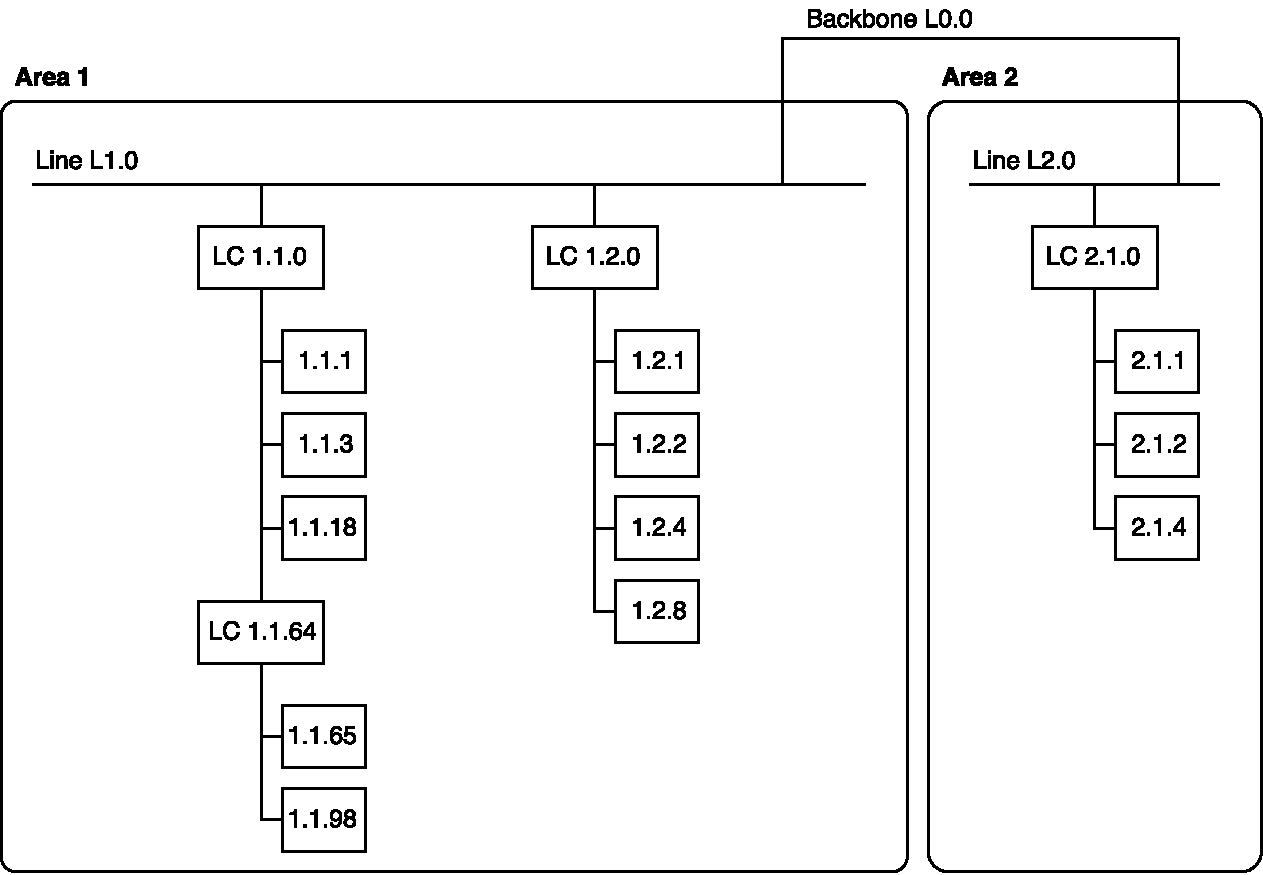
\includegraphics[width=\textwidth]{figures/100-knx-demo-topo.pdf}
	\caption[KNX network topology]{Exemplary logical topology of a \gls{knx} network with line couplers (LC) and normal devices.}
	\label{fig:background:knx:topo}
\end{figure}

The logical structure builds on top of the physical topology and is intended to remodel the functional structure of buildings in a logical tree topology. This tree topology is divided into three levels: areas, lines, and devices. Each device or node is assigned a physical address, defining area, line, and device number. (cf. Table~\ref{tab:background:bas:knx:topo:addr})
Each device is directly connected to a line, which can accommodate up to 256 devices, if supported by all devices on the line. Alternatively, up to 64 devices can be in one line segment before line repeater is required. (cf. Table~\ref{tab:background:bas:knx:topo:tpsegments})
Most \gls{knx} devices still follow the TP1-64 specification. Due to the high market fragmentation devices are often not mark in regards of supporting either TP1-64 or TP1-256, therefore it is still recommended to only use 64 devices within a line segment. \alert{sentence too long?} Thus, a full logical line is advised to be build using three line repeater. \parencite{Sokollik2017,Merz2009}

\begin{table}
	\aboverulesep=0ex
	\belowrulesep=0ex
	\renewcommand{\arraystretch}{1.2}
	
	\centering
	\begin{tabular}{|l|r|r|}
		\toprule
		& \textbf{TP1-64} & \textbf{TP1-256} \\\midrule
		maximum devices per segment & 64 & 256 \\
		maximum distance between 2 devices & 700m & 700m \\
		maximum length of a physical line & 1000m & 1000m \\
		\bottomrule
	\end{tabular}
	\caption[Segment properties for \knx.TP1-64 and \knx.TP1-256]{Segment properties for \knx.TP1-64 and \knx.TP1-256. cf. \textcite{Sokollik2017}}
	\label{tab:background:bas:knx:topo:tpsegments}
\end{table}

Usually a line coupler is installed as a line repeater. A line coupler is an active device to connect one logical level of the \gls{knx} network to another one, which can be one line segment to another line segment.
However, their original purpose is to separate the different levels of the logical \gls{knx} topology, explicitly to attach a line to the main line of an area or to attach a main line to the backbone. (cf. Figure~\ref{fig:background:knx:topo})
An area is formed by combining up to 16 lines: one main line and 15 sub-lines. All main lines are then connected to a backbone line, again via area couplers. \parencite{Sokollik2017}

As active devices line couplers are assigned addresses, and are able to filter traffic by addresses similar to \gls{ip} router. %usually with device number 0 in case it connects a line to backbone line.
Further couplers provide galvanic isolation to mitigate damages by high voltages, shorted circuits, etc. As a result multiple power supplies are required, basically one for each line segment.
An important feature to be aware of, when using line couplers, is that a \gls{knx} telegram can only be routed over six hops. This was introduced to prevent high network load in case of cyclic routing, comparable to the time to live in IP based networks. \parencite{Sokollik2017}

% KNX Address byte-field

\begin{table}[h]
	\aboverulesep=0ex
	\belowrulesep=0ex
	\renewcommand{\arraystretch}{1.2}
	
	\centering
	\begin{tabular}{|l|c|c|c|c|c|c|c|c|c|c|c|c|c|c|c|c|}
		\toprule
		Byte & \multicolumn{8}{c|}{1} & \multicolumn{8}{c|}{0} \\\midrule
		Bit & 7 & 6 & 5 & 4 & 3 & 2 & 1 & 0 & 7 & 6 & 5 & 4 & 3 & 2 & 1 & 0\\\midrule
		Physical Address & \multicolumn{4}{c|}{area} & \multicolumn{4}{c|}{line} & \multicolumn{8}{c|}{device}\\\midrule
		Group Address & \multicolumn{5}{c|}{main} & \multicolumn{3}{c|}{middle} & \multicolumn{8}{c|}{sub group}\\
		\bottomrule
	\end{tabular}
	\caption[Bit field for KNX addresses]{Bit field for \acs{knx} addresses. Only the most common used three-level group address is shown here. cf.~\textcite{Merz2009,Sokollik2017} }
	\label{tab:background:bas:knx:topo:addr}
\end{table}

Additional to the physical address each devices is assigned, devices may listen to group addresses.
\todo{describe layers/modes of group addresses?}
Whereby physical addresses are used to communicate with one specific device, which is common during installation, throughout normal operation mostly group addresses are used. As the name implies multiple devices may listen to such an address, allowing one light switch to turn on or off multiple lights for instance.

% ------------------------------------------------------------------------------	
\subsubsection{KNX Protocol}
\label{sec:background:bas:knx:proto}

\begin{comment}
		\begin{itemize}
		\item 3 types of telegrams \parencite{Hubner2009} \parencite{Merz2009}
			\subitem data - "sent in response to an individual action such as" \parencite{Merz2009} pressing a button (standard and extended \parencite{Hubner2009})
			\subitem acknowledge - "All devices (receivers) that belong to this group simultaneously confirm that they have received the data frame by returning an acknowledgment frame." \parencite{Merz2009}
			\subitem poll - "one device can query 1-Byte-Information from up to 15 other devices. Addressing is done via group addresses" \parencite{Hubner2009}
		\item Standard Data Telegram
			\subitem cf. Table~\ref{tab:background:bas:knx:proto:knx-standard}
		\item Extended Data Telegram
			\subitem cf. Table~\ref{tab:background:bas:knx:proto:knx-extended}
		\item Poll Telegram
			\subitem cf. Table~\ref{tab:background:bas:knx:proto:knx-poll}
		\item Acknowledge Telegram
			\subitem cf. Table~\ref{tab:background:bas:knx:proto:ack}
	\end{itemize}
\end{comment}

To communicate within a \gls{knx} network, devices send telegrams in their line. Due to the topology (cf. Section~\ref{sec:background:bas:knx:topo}) and technological nature of \gls{knx} these telegrams are always broadcasted within the respective line, only line couplers may narrow down the scope in which a specific telegram might be received. Telegrams are very comparable to packets in an IP network.

Within the \gls{knx} specification three types of telegrams are defined: Data Telegrams, Poll Telegrams, and Acknowledge Telegrams. (cf. Table~\ref{tab:background:bas:knx:proto:knx-standard},~\ref{tab:background:bas:knx:proto:ctrle},~\ref{tab:background:bas:knx:proto:knx-poll}, and~\ref{tab:background:bas:knx:proto:ack})
Each of which can be transmitted using on of four priorities, which are show in Table~\ref{tab:background:bas:knx:proto:prio}. Hereby it is to note, that a logical 0 is the dominant symbol. Consequently, the priority encoding is designed in a way, that lower priority telegrams are overruled by telegram with higher priority.
The bus devices detect these collisions and avoid them by following the \gls{csmaca} principle.

The telegram type is encoded in the first two bit of the \gls{ctrl} byte, which functions as a header of a \gls{knx} telegram. Next to the type it also contains a repeat flag, an acknowledge flag, and the priority. (see Figure~\ref{tab:background:bas:knx:proto:ctrl})

% KNX prio table

\begin{table}
	\aboverulesep=0ex
	\belowrulesep=0ex
	\renewcommand{\arraystretch}{1.2}
	\newcolumntype{Y}{>{\centering\arraybackslash}X}
	
	\centering
	\begin{tabularx}{0.7\textwidth}{|l|Y|Y|}
		\toprule
		Bit & 1 & 0 \\\midrule
		Function & \multicolumn{2}{c|}{Priority} \\\bottomrule
		\toprule
		System priority & 0 & 0 \\\midrule
		Alarm priority & 1 & 0 \\\midrule
		High priority & 0 & 1 \\\midrule
		Low priority & 1 & 1 \\\bottomrule
	\end{tabularx}
	\caption[\knx priority encoding]{\knx priority encoding. cf.~\textcite{Merz2009}}
	\label{tab:background:bas:knx:proto:prio}
\end{table}

%\subsubsection{Data Telegram}
\paragraph{Data Telegram}
\label{sec:background:bas:knx:proto:data}

The data telegram being utilised the most and used for transferring commands, state, and value changes, comes in two flavours.
The standard data telegram (cf. Table~\ref{tab:background:bas:knx:proto:knx-standard}) is able to transmit between 2 and 16 bytes per telegram. To transfer more data the extended data telegram (cf. Table~\ref{tab:background:bas:knx:proto:knx-extended}) can be utilised, which can transfer up to 255 bytes.
Both are sent in reaction of an direct interaction (e.g. light switch) or to send periodical sensor data (e.g. temperature). \parencite{Merz2009}
Once received and successfully processed, the recipient replies then with an acknowledge telegram. \parencite{Merz2009,Sokollik2017}

The extended data telegram introduces another header byte after \gls{ctrl}, the \gls{ctrle} header byte. It contains information otherwise encoded together with the payload length like the destination address type and the hop count, thus it allows the payload length to encoded as a full byte, ranging up to 255. (see Table~\ref{tab:background:bas:knx:proto:ctrle})

% KNX data telegram structure for standard and extended

\begin{table}
	\aboverulesep=0ex
	\belowrulesep=0ex
	\renewcommand{\arraystretch}{1.2}
	\newcolumntype{Y}{>{\centering\arraybackslash}X}
	
	\centering
	\begin{tabularx}{\textwidth}{|l|Y|Y|Y|Y|Y|Y|Y|Y|Y|Y|Y|Y|Y|Y|Y|Y|Y|Y|Y|Y|Y|Y|Y|Y|}
		\toprule
		Byte & \multicolumn{8}{c|}{0} & \multicolumn{8}{c|}{1} & \multicolumn{8}{c|}{2} \\\midrule
		Bit & & & & & & & & & & & & & & & & & & & & & & & & \\\midrule
		Function & \multicolumn{8}{c|}{CTRL} & \multicolumn{16}{c|}{Source Address} \\\bottomrule
		\toprule
		Byte & \multicolumn{8}{c|}{3} & \multicolumn{8}{c|}{4} & \multicolumn{8}{c|}{5} \\\midrule
		Bit & & & & & & & & & & & & & & & & & & & & & & & & \\\midrule
		Function & \multicolumn{16}{c|}{Destination Address} & \multicolumn{1}{c|}{\parbox[t][26pt][s]{0.2cm}{A T}} & \multicolumn{3}{c|}{Hops} & \multicolumn{4}{c|}{Length} \\\bottomrule
		\toprule
		Byte & \multicolumn{8}{c|}{6} & \multicolumn{8}{c|}{$7+n$} & \multicolumn{8}{c|}{$8+n$} \\\midrule
		Bit & & & & & & & & & & & & & & & & & & & & & & & & \\\midrule
		Function & \multicolumn{16}{c|}{Payload $n+1$ Bytes} & \multicolumn{8}{c|}{Parity} \\\bottomrule
	\end{tabularx}
	\caption[Standard \knx data telegram]{Standard \knx data telegram with $2$ to $16$ bytes of payload. Control Byte (CTRL) cf. Table~\ref{tab:background:bas:knx:proto:ctrl}, Source Address, Destination Address cf. Table~\ref{tab:background:bas:knx:topo:addr}, Address Type (AT), Hop Count (Hops), Payload Length (Length), Payload, and Parity.}
	\label{tab:background:bas:knx:proto:knx-standard}
\end{table}

\begin{table}
	\aboverulesep=0ex
	\belowrulesep=0ex
	\renewcommand{\arraystretch}{1.2}
	\newcolumntype{Y}{>{\centering\arraybackslash}X}
	
	\centering
	\begin{tabularx}{\textwidth}{|l|Y|Y|Y|Y|Y|Y|Y|Y|Y|Y|Y|Y|Y|Y|Y|Y|Y|Y|Y|Y|Y|Y|Y|Y|}
		\toprule
		Byte & \multicolumn{8}{c|}{0} & \multicolumn{8}{c|}{1} & \multicolumn{8}{c|}{2} \\\midrule
		Bit & & & & & & & & & & & & & & & & & & & & & & & & \\\midrule
		Function & \multicolumn{8}{c|}{CTRL} & \multicolumn{8}{c|}{CTRLE} & \multicolumn{8}{c|}{Source Address} \\\bottomrule
		\toprule
		Byte & \multicolumn{8}{c|}{3} & \multicolumn{8}{c|}{4} & \multicolumn{8}{c|}{5} \\\midrule
		Bit & & & & & & & & & & & & & & & & & & & & & & & & \\\midrule
		Function & \multicolumn{8}{c|}{Source Address} & \multicolumn{16}{c|}{Destination Address} \\\bottomrule
		\toprule
		Byte & \multicolumn{8}{c|}{6} & \multicolumn{8}{c|}{$7$} & \multicolumn{8}{c|}{$8+n$} \\\midrule
		Bit & & & & & & & & & & & & & & & & & & & & & & & & \\\midrule
		Function & \multicolumn{8}{c|}{Length} & \multicolumn{16}{c|}{Payload $n+1$ Bytes} \\\bottomrule
		\toprule
		Byte & \multicolumn{8}{c|}{$9+n$} & \multicolumn{16}{c|}{ } \\\cmidrule{1-9}
		Bit & & & & & & & & & \multicolumn{16}{c|}{ } \\\cmidrule{1-9}
		Function & \multicolumn{8}{c|}{Parity} & \multicolumn{16}{c|}{ } \\\bottomrule
	\end{tabularx}
	\caption[Extended \knx data telegram]{Extended \knx data telegram with $2$ to $255$ bytes of payload. Control Byte (CTRL) cf. Table~\ref{tab:background:bas:knx:proto:ctrl}, Extended Control Byte (CTRLE) cf. Table~\ref{tab:background:bas:knx:proto:ctrle}, Source Address, Destination Address cf. Table~\ref{tab:background:bas:knx:topo:addr}, Payload Length (Length), Payload, and Parity.}
	\label{tab:background:bas:knx:proto:knx-extended}
\end{table}
% KNX telegram CTRL byte

\begin{table}
	\aboverulesep=0ex
	\belowrulesep=0ex
	\renewcommand{\arraystretch}{1.2}
	\newcolumntype{Y}{>{\centering\arraybackslash}X}
	
	\centering
	\begin{tabularx}{\textwidth}{|l|Y|Y|Y|Y|Y|Y|Y|Y|}
		\toprule
		Byte & \multicolumn{8}{c|}{0} \\\midrule
		Bit & 7 & 6 & 5 & 4 & 3 & 2 & 1 & 0 \\\midrule
		Function & \multicolumn{2}{c|}{TT} & R & A & \multicolumn{2}{c|}{P} & \multicolumn{2}{c|}{reserved} \\\bottomrule \toprule
		Standard Data Telegram & 1 & 0 & R & 1 & \multicolumn{2}{c|}{P} & \multicolumn{2}{c|}{ } \\\midrule
		Extended Data Telegram & 0 & 0 & R & 1 & \multicolumn{2}{c|}{P} & \multicolumn{2}{c|}{ } \\\midrule
		Poll Telegram & 1 & 1 & 1 & 1 & 0 & 0 & \multicolumn{2}{c|}{ } \\\midrule
		Acknowledge Telegram & \multicolumn{2}{c|}{ } & 0 &0 & \multicolumn{2}{c|}{ } & \multicolumn{2}{c|}{ } \\\bottomrule
	\end{tabularx}
	\caption[\knx CTRL Byte]{\knx CTRL Byte. Telegram Type (TT), Repeat (R), Acknowledge (A), and Priority (P). cf. \textcite{Sokollik2017}}
	\label{tab:background:bas:knx:proto:ctrl}
\end{table}
% KNX CTRL-Extended control byte

\begin{table}[p]
	\aboverulesep=0ex
	\belowrulesep=0ex
	\renewcommand{\arraystretch}{1.2}
	\newcolumntype{Y}{>{\centering\arraybackslash}X}
	
	\centering
	\begin{tabularx}{0.7\textwidth}{|l|Y|Y|Y|Y|Y|Y|Y|Y|}
		\toprule
		Byte & \multicolumn{8}{c|}{0} \\\midrule
		Bit & 7 & 6 & 5 & 4 & 3 & 2 & 1 & 0 \\\midrule
		Function & AT & \multicolumn{3}{c|}{Hops} & \multicolumn{4}{c|}{EFF} \\\bottomrule
	\end{tabularx}
	\caption[\knx CTRLE Byte]{\knx CTRLE Byte. Address Type (AT), Hop Count, and Extended Frame Format (EFF). cf. \textcite{Sokollik2017}}
	\label{tab:background:bas:knx:proto:ctrle}
\end{table}

%\subsubsection{Acknowledge Telegram}
\paragraph{Acknowledge Telegram}
\label{sec:background:bas:knx:proto:ack}

The acknowledge telegram can indicate the correct reception (\code{ACK}, positive acknowledge), faulty reception (\code{NACK}, negative acknowledge), or that the receiving device is currently busy and is not able to process the telegram. (cf. Table~\ref{tab:background:bas:knx:proto:ack})
It consists of one byte and is sent by the recipient after waiting 13 bit times.
If the sender receives an positive acknowledge, the telegram was send successfully and no further action is required. However, if it detects an negative acknowledge or busy signal, the telegram is resend up to three times.
Supposed a busy signal occurred, the sender adds a waiting period before attempting to resend the telegram.
Given, the sender does not receives any form of acknowledge telegram within 13 bit times, it resends the telegram also up to three times.
In case the sender addressed the original telegram to multiple devices by using a group address as destination, the acknowledge frame is send simultaneously by all recipients. Due to the bus characteristic of being normally high (1), an negative acknowledge or busy signal overrules a positive acknowledge, since \code{BUSY} and \code{NACK} are encoded with low bits (0). \parencite{Merz2009,Sokollik2017}

\begin{table}[p]
	\aboverulesep=0ex
	\belowrulesep=0ex
	\renewcommand{\arraystretch}{1.2}
	\newcolumntype{Y}{>{\centering\arraybackslash}X}
	
	\centering
	\begin{tabularx}{0.7\textwidth}{|l|Y|Y|Y|Y|Y|Y|Y|Y|}
		\toprule
		Byte & \multicolumn{8}{c|}{0} \\\midrule
		Bit & 7 & 6 & 5 & 4 & 3 & 2 & 1 & 0 \\\bottomrule
		\toprule
		ACK  & 1 & 1 & 0 & 0 & 1 & 1 & 0 & 0 \\\midrule
		NACK & 0 & 0 & 0 & 0 & 1 & 1 & 0 & 0 \\\midrule
		BUSY & 1 & 1 & 0 & 0 & 0 & 0 & 0 & 0 \\\midrule
		NACK + BUSY & 0 & 0 & 0 & 0 & 0 & 0 & 0 & 0 \\\bottomrule
	\end{tabularx}
	\caption[KNX acknowledge telegram]{\gls{knx} short acknowledge telegram.}
	\label{tab:background:bas:knx:proto:ack}
\end{table}

%\subsubsection{Poll Telegram}
\paragraph{Poll Telegram}
\label{sec:background:bas:knx:proto:poll}

The poll telegram allows to poll one byte of data from up to 15 devices, however, it is seldom used in \gls{knx} networks. It consists of a poll data request frame (cf. Table~\ref{tab:background:bas:knx:proto:knx-poll}) and a poll data response frame. Former starts the poll telegram and sets the group address to query, also it defines how many bytes to receive.
The poll data response consists of each device sending one byte on the bus without starting a new telegram. The responding devices are doing so in a prior configured time slot. \parencite{Hubner2009,DIN_EN_50090-5-2}

\begin{table}[p]
	\aboverulesep=0ex
	\belowrulesep=0ex
	\renewcommand{\arraystretch}{1.2}
	\newcolumntype{Y}{>{\centering\arraybackslash}X}
	
	\centering
	\begin{tabularx}{\textwidth}{|l|Y|Y|Y|Y|Y|Y|Y|Y|Y|Y|Y|Y|Y|Y|Y|Y|Y|Y|Y|Y|Y|Y|Y|Y|}
		\toprule
		Byte & \multicolumn{8}{c|}{0} & \multicolumn{8}{c|}{1} & \multicolumn{8}{c|}{2} \\\midrule
		Bit & & & & & & & & & & & & & & & & & & & & & & & & \\\midrule
		Function & \multicolumn{8}{c|}{CTRL} & \multicolumn{16}{c|}{Source Address} \\\bottomrule
		\toprule
		Byte & \multicolumn{8}{c|}{3} & \multicolumn{8}{c|}{4} & \multicolumn{8}{c|}{5} \\\midrule
		Bit & & & & & & & & & & & & & & & & & & & & & & & & \\\midrule
		Function & \multicolumn{16}{c|}{Destination Address} & \multicolumn{4}{c|}{ } & \multicolumn{4}{c|}{poll data} \\\bottomrule
		\toprule
		Byte & \multicolumn{8}{c|}{6} & \multicolumn{16}{c|}{ } \\\cmidrule{1-9}
		Bit & & & & & & & & & \multicolumn{16}{c|}{ } \\\cmidrule{1-9}
		Function & \multicolumn{8}{c|}{Parity} & \multicolumn{16}{c|}{ } \\\bottomrule
	\end{tabularx}
	\caption[KNX poll telegram]{\gls{knx} poll telegram. Control Byte (CTRL) cf. Table~\ref{tab:background:bas:knx:proto:ctrl}, Source Address, Destination Address cf. Table~\ref{tab:background:bas:knx:topo:addr}, expected length of poll data (poll data), and Parity.}
	\label{tab:background:bas:knx:proto:knx-poll}
\end{table}

\subsubsection{KNX Communication}
\label{sec:background:bas:knx:communication}

\begin{comment}
		\begin{itemize}
		\item application layer described in \textcite{DIN_EN_50090-4-1}
		\item communication modes \parencite{DIN_EN_50090-4-1}
			\subitem point-to-multipoint, connection-less (multicast)
			\subitem point-to-domain, connection-less (broadcast)
			\subitem point-to-all-points, connection-less (system broadcast)
			\subitem point-to-point, connection-less
			\subitem point-to-point, connection-oriented
		\item APCI describes operation on application layer
		\item Response need to match the Request APCI type and must be send on the corresponding communication mode allowed for this packet. cf. \textcite[][page 9--10]{DIN_EN_50090-4-1}
	\end{itemize}
\end{comment}

Apart from the basic \gls{knx} protocol (cf. Section~\ref{sec:background:bas:knx:proto}), which is comparable to the data link layer in the \gls{osi} model, the \textcite{DIN_EN_50090-4-1} describes two layers on top: a transport layer and an application layer.
However, it is to note, that even when official \gls{knx} specification draws parallels to the \gls{osi} model, a direct comparison to the \gls{osi} model as seen in \gls{ip} networks is difficult, due to the reduced complexity of the protocol stack in \gls{knx}.

The transport layer defines multiple transport layer services, which are encoded in the \gls{tpci} (cf. Table~\ref{tab:background:bas:knx:comm:tpci-apci}) and can be clustered into five categories or modes:

\begin{enumerate}
	\item point-to-multipoint, connection-less (multicast)
	\item point-to-domain, connection-less (broadcast)
	\item point-to-all-points, connection-less (system broadcast)
	\item point-to-point, connection-less
	\item point-to-point, connection-oriented
\end{enumerate}
\parencite[p.~30]{DIN_EN_50090-4-2}

Depending on the category, multiple telegrams might be send in order to establish a connection, e.g. point-to-point, connection oriented.
Further, these communication modes are used by the 44 different application layer services described in \textcite{DIN_EN_50090-4-1}.
These application layer services can be used to access and set device states, encoded in \glspl{dpt}, or to configure the device.
Each response needs to match the requests \gls{apci} type and must be send on with the corresponding communication mode allowed for this telegram. \parencite[pp.~9--10]{DIN_EN_50090-4-1}

\glspl{dpt}, in turn, define the structure of the data, which is transported using the application layer services.
They are defined to consist of a combination of a data type and a dimension. Whereby the former is required to specify format and encoding. The later, however, defines range and unit.
It was decided not to specify data types and dimensions separately to reduce abstract naming and confusion.
Therefore any \gls{dpt} declares a single combination of format, encoding, range, and unit. \parencite[p.~38]{DIN_EN_50090-3-3}

Each \gls{dpt} is identified by an 16 bit main number and an 16 bit sub-number, separated by a dot. The main number describes the format and encoding and consequently the sub-number describes range and unit. As a result, \glspl{dpt} with the same main number share the format and encoding.

\begin{table}
	\aboverulesep=0ex
	\belowrulesep=0ex
	\renewcommand{\arraystretch}{1.2}
	\newcolumntype{Y}{>{\centering\arraybackslash}X}
	
	\centering
	\begin{tabularx}{\textwidth}{|l|Y|Y|Y|Y|Y|Y|Y|Y|Y|Y|Y|Y|Y|Y|Y|Y|}
		\toprule
		Byte & \multicolumn{8}{c|}{6} & \multicolumn{8}{c|}{7} \\\midrule
		Bit & & & & & & & & & & & & & & & & \\\midrule
		\multirow{2}{*}{Function} & \multicolumn{6}{c|}{TPCI} & \multicolumn{10}{c|}{APCI} \\\cmidrule{2-7}
		 & DC & No & \multicolumn{4}{c|}{Seq. Number} & \multicolumn{10}{c|}{} \\\bottomrule
	\end{tabularx}

	\caption[KNX TPCI/APCI structure in a standard data telegram]{\gls{knx} \acrshort{tpci}/\acrshort{apci} structure in a standard data telegram. Data/Control flag (DC), Numbered/Unnumbered flag (No), Sequence Number (Seq. Number).}
	\label{tab:background:bas:knx:comm:tpci-apci}
\end{table}
	
\subsubsection{KNX Management Procedures}
\label{sec:background:bas:knx:management}

\begin{comment}
	\begin{itemize}
		\item "describe the device independent management procedures" \parencite{DIN_EN_50090-7-1}
		\item "shall be used to configure the network, and to get the information about the configuration of the network and connected devices" \parencite{DIN_EN_50090-7-1}
		\item " no knowledge of the single devices is required. They will work with every device connected to the network" \parencite{DIN_EN_50090-7-1}
		\item "shall be based on the use of the dedicated application layer services which are specified in EN 50090-4-1 \parencite{DIN_EN_50090-4-1} for this purpose" \parencite{DIN_EN_50090-7-1}
	\end{itemize}
\end{comment}

To ensure maximum compatibility among \gls{knx} devices of different vendors, it is not only sufficient these devices implement the same protocol stack (cf. Section~\ref{sec:background:bas:knx:proto}) and use the same communication services (cf. Section~\ref{sec:background:bas:knx:communication}).
Moreover, it is also required that they share a common set of management and configuration services.
This is especially true in an environment like \gls{knx}, where devices need to be fully interchangeable and need to be configurable by a common tool used by electricians.

Therefore, the \gls{knx-assoc} specified two sets of management procedure.
For these procedures dedicated application layer services were defined in \textcite{DIN_EN_50090-4-1}. (cf. Section~\ref{sec:background:bas:knx:communication})
The first, being called network management procedures, are device independent, which do not require any knowledge or insight of the devices and will work across all vendors and device types. \parencite[pp.~11~ff.]{DIN_EN_50090-7-1}
They mainly provide routines to configure addresses, read serial numbers, get functions, or to find all devices in programming mode.

Secondly, there are device management procedures, which require in depth knowledge of the devices. \parencite[pp.~30~ff.]{DIN_EN_50090-7-1}
These are used to i.e. configure devices, restart them, and verify the configuration.

\subsubsection{Security in KNX}
\label{sec:background:bas:knx:security}

\begin{comment}
	\begin{itemize}
		\item copulers allow filtering 
			\subitem "This means that data frames transmitted by a sender are only forwarded to recipients that are not on the sender’s line." \parencite{Merz2009}
			\subitem "The filter function only forwards data frames to where they are needed. This reduces the overall amount of data frame traffic and keeps the data traffic on one line separate from the data traffic on another line, allowing data to be transferred on several lines simultaneously." \parencite{Merz2009}
		\item main group 14 and 15 should not be used \parencite{Hubner2009}
			\subitem can not be filtered due to limited space for filter tables in couplers \parencite{Hubner2009}
			
		\item cf DIN50090-3-4 page 13 (secure application layer) \parencite{DIN_EN_50090-3-4}
	\end{itemize}
\end{comment}

With \gls{knx} being so widely used, it is also deployed in security sensitive areas like access control\footnote{\url{http://search-ext.abb.com/library/Download.aspx?DocumentID=2CDC500074M0201&LanguageCode=en&DocumentPartId=&Action=Launch}}, ventilation, or fire alarms\footnote{\url{https://www.knx.org/media/docs/downloads/Marketing/Flyers/KNX-Solutions/KNX-Solutions_en.pdf}}.
As a consequence it is only sensible to consider not only the operational safety, but also the information security of \gls{knx} networks. Meaning, it should not only be assured, that the network is operational at any time, but it needs to be protected against malicious usage or intrusion.
This is especially vital, if gateways to \gls{ip} networks exists as these are easily exposed to the internet.

By design \gls{knx} introduces a zone concept by distinguishing between lines and areas.
This offers the possibility to limit a potential attack to just one line, because the traffic between lines is filtered by line couplers.
This filter function ensures, that only traffic concerning devices in other lines is routed to the main or backbone line.

However, filtering traffic comes with certain limitations. For instance the line couplers need be configured properly, which can be done automatically by the installation and configuration Software \gls{ets}. \parencite{Merz2009}
Further, to ensure proper filtering the main groups 14 and 15 must not be used, since they cannot be filtered, due to limited space for filter tables in couplers. \parencite{Hubner2009}
Moreover, traffic within the affected line can still be red and manipulated by an attacker, as well as device can be reconfigured or attacked.

Another possibility to secure a \gls{knx} network is to enable \gls{s-al}, as defined in \textcite{DIN_EN_50090-3-4}. \Gls{s-al} is an extension of the \gls{knx} specification defining an encrypted application layer (cf. Section~\ref{sec:background:bas:knx:communication}) for multicast and point-to-point communication, which can be used next to normal unencrypted traffic.
As encryption standard \textcite{DIN_EN_50090-3-4} defines \acs{aes}-128 in \gls{ctr} or \gls{ccm} mode.
Later also functions as authentication. \todo{ensure short formes are used, at least for AES}

Nonetheless it is to note, that \textcite{DIN_EN_50090-3-4} is merely a draft at the point of June 2017.
Therefore, it is not to expect, that available \gls{knx} devices with this capability will be on the market any time soon. This may also be caused by the relatively high life time of devices which are installed permanently in buildings, which have an expected lifetime of up to 40 years.


% ------------------------------------------------------------------------------
%\section{\lonworks}

%\section{\bacnet}
	
	\chapter{Network Analysis and Netflow}
	% background about netflow
	\label{sec:background:network}
	% !TeX spellcheck = en_GB

\todo{general introductory sentence about network mon}

\subsection{Intrusion Detection Systems (IDS)}
\label{sec:background:network:ids}

\begin{comment}
		\begin{itemize}
		\item \enquote{A good network intrusion detection system (IDS) can have an enormous positive impact on the overall security of your oragnization} \parencite{Northcutt2005}
		\item \enquote{By detecting malicious activity, network intrusion detection enables you to identify and react to threats against your environment, as well as threasts that your hosts might be directing at hosts on other networks.} \parencite[p. 201]{Northcutt2005}
		\item \enquote{Without intrusion detection, you may never know about an attack that doesn't damage your host, but simply extracts information[...]. Without intrusion detection, you will be unaware of these events until it's much too late.} \parencite[p. 202]{Northcutt2005}
		\item Not only identifies attacks, but also reveals attack attempts and probing \parencite[p. 202]{Northcutt2005}
		\item 
	\end{itemize}
\end{comment}

Good network security consists of many parts, covering a huge variety of methods and functions. \hint{This sounds weird and artificial.}
As one of these parts \enquote{a good \gls{ids} can have an enormous positive impact on the overall security [...]}. \parencite{Northcutt2005}
The basic idea is to monitor the network traffic passing by sensors and therefore be able to detect malicious activities.
This allows the \gls{ids} to detect and identify threasts against the own environment or theats ones own hosts impose to other environments, due to an infection with malware.
Without intrusion detection one might never detect attacks, that do not influence normal operations but for instance extract information.

Further, \gls{ids} may also identify attack attempts and probing, allowing to further harder the environment and take precautions.

Nowadays \glspl{ids} are a commonly deployed in \gls{ip} networks. There are different kinds of \glspl{ids}, which can be discriminated by working principle. The following section is giving an overview of the most common technologies. \parencite[cf.][pp.~201-202]{Northcutt2005}

\subsubsection{Signature-based Intrusion Detection Systems (SIDS)}
\label{sec:background:network:ids:sig}

\begin{comment}
	\begin{itemize}
		\item \enquote{[...] IDS signature is a pattern you are looking for in traffic.} \parencite{Northcutt2005}
		\item \enquote{When a signature for an attack matches observed traffic, an alert is generated, or the event is otherwise recorded.} \parencite{Northcutt2005}
		\item \enquote{Many signatures are protocol or application specific;} \parencite{Northcutt2005}
		\item requires to update a curated set of signatures regularly \parencite{Northcutt2005}
		\item \enquote{Signature development is always a balancing act. A specific signature might be extremely accurate in identifying a particular attack [...] [but] If an attacker slightly modifies the attack, the signature might not be able to identify it at all.} \parencite{Northcutt2005}
			\subitem precision/recall balance
		\item \enquote{Every intrusion detection system generates false positives.} \parencite[p.~205]{Northcutt2005}
		\item \enquote{By selecting a solid IDS product and tuning your sensors, you can reduce false positives, but you can't completely eliminate them.} \parencite[p.~205]{Northcutt2005}
		\item \enquote{[...], but each false negative is a legitimate attack or incident that IDS failed to notice.} \parencite[p.~206]{Northcutt2005}
		\item \enquote{Besides false positives, you might also have alerts that address legitimate problems that you simply don't care about.} (Unwanted Alerts) \parencite[p.~206]{Northcutt2005}
		\item 
	\end{itemize} 
\end{comment}

One of the more traditional \gls{ids} principles are signature based systems.
They work by comparing patterns (signatures) of malicious traffic to the observed traffic. When a pattern matches an alert is raised.
This requires many protocol and application specific signatures, which are difficult to create and maintain, since a good balance between being too generic and being too specific needs to be found.

A signature which is too generic, may cause many false positives. This might lead to an elimination of any positive effect of the \gls{ids}, since real alerts become impossible to spot among the false positives.
In contrast, however, a signature which is too specific might suffer from a too narrow scope. Meaning, that it might be really precise in classifying one particular attack, but fails to do so if an attacker just slightly modifies it.

As a result, a valuable \gls{ids} solution is characterised by an balanced precision/recall ratio. This can be archived by using a good signature database and fine tuning the sensors.
However, it is to note, that every \gls{ids} will produce false positives. This derives out of the consideration, that each false negative is an legitimate attack, which was not detected. Therefore a slight tendency to (over) sensitivity is sensible.

Other than false positives, there might be legitimate alerts that are of no interest. These unwanted alerts should be blocked, to not numb \alert{(is this the right word here?)} the system administrator. \parencite[cf.][pp.~205-206]{Northcutt2005}
	
\subsubsection{Anomaly-based Intrusion Detection Systems (ABIDS)}
\label{sec:background:network:ids:anomaly}
	
\begin{comment}
	\begin{itemize}
		\item \enquote{establishing baselines of normal network activity over a period of time, then detecting significant deviations from the baseline.} \parencite[p. 203]{Northcutt2005}
		\item \enquote{[...] later, if the IDS sensor sees a high volume of traffic involving a previously unused service on a host, this could indicate a distributed denial of service (DDoS) attack against the host or a compromised host providing a new service.} \parencite{Northcutt2005}
		\item \enquote{[...] drawback of this type of anomaly detection is that the baseline needs to be updated constantly to reflect authorized changes[...]} \parencite{Northcutt2005}
		\item \enquote{If the baseline can be kept current, or if the environment is quite static and the baseline changes rarely, anomaly detection can be extremely effective at identifying certain types of attacks [...]} \parencite{Northcutt2005}
		\item \textbf{\enquote{Unfortunately, this type of anomaly detection cannot identify most other types of attacks, so it is best used to complement other IDS technologies.}} \parencite{Northcutt2005}
		\item \enquote{[...] can [...] identifying certain previously unknown instances of attacks [...]} \parencite{Northcutt2005}
		\item \enquote{cannot determine the intent of an attack} \parencite{Northcutt2005}
	\end{itemize}
\end{comment}

Another major technology used in \glspl{ids} is anomaly detection. (cf. Section~\ref{sec:background:network:novelty})
Unlike signature based methods (cf. Section~\ref{sec:background:network:ids:sig}) it does not require an predefined set of rules, rather deploying anomaly detection it is able to auto-generate rules specific for the monitored network and then perform whitelisting using these rules.

This is archived by having a so called training phase before deploying the \gls{ids}. During the training phase a baseline model is established using the normal network activity over period of time. It is to note, that this period should be long enough to cover normally recurring usage cycles, e.g. day-time/night-time, weekday/weekends, etc.

After an successful training phase the \gls{ids} uses the generated baseline model to compare bypassing traffic against it.
If it detects a significant deviation from it, an alert is raise as it indicates unusual network activities.
For instance, if an internal host in an \gls{ip} network, produces suddenly a lot of outbound traffic, which was not the case before, it might indicate an infection on this host.

This example illustrates 2 primary drawbacks of purely anomaly-based \glspl{ids}: 
First, the system can not identify which kind of attack it detects, it merely identifies an anomaly. To identify the intention of the attack it would need to be combined with a rule system or signature-based approach.

Second, the increased outbound traffic in the example could have been generated by a new legitimate software, i.e. a website crawler.
Consequently, strictly separated training and operational phases lead to poor adaption of the \gls{ids} to a changing environment.
This could be mitigated by updating the baseline model during normal operation, so t accommodates for changes.
However, by continuing the training phase, attacker might be able to reprogram the baseline in their favour by injecting malicious packets very rarely at the beginning, but then increase the amount steadily.
By doing so the relative deviation from the continuing trained baseline model stays relatively low and will therefore not trigger an alert.
This means, the decision if the baseline model should be trained continuously has to be made under careful consideration of the nature of the network to be monitored.

All in all, anomaly-based \glspl{ids} are ideal to identify prior unknown threats and attacks in relatively stable environments. However, it might also identify (legitimate) changes in the environment as anomaly. Additionally it might be unable to detect attacks which mimic regular behaviour and only deviate slightly from legitimate traffic.
As a result, anomaly-based \glspl{ids} should be combined with other \gls{ids} technologies, when used to protect production systems.
\parencite[cf.][pp.~203-204]{Northcutt2005} \todo{check pages}
	
\subsubsection{State-based Intrusion Detection Systems\hint{??}}
\label{sec:background:network:ids:state}

\begin{itemize}
	\item cf. \textcite{Whitman2009} page 306 
\end{itemize}

% ------------------------------------------------------------------------------
\subsection{Flow Monitoring}
\label{sec:background:network:netflow}

\begin{comment}
	\begin{itemize}
		\item active
			\begin{itemize}
				\item inject additional traffic to measure things \parencite{Hofstede2014}
				\item e.g. ping, traceroute
			\end{itemize}
		\item passive
			\begin{itemize}
				\item "observe existing traffic as it passes by" \parencite{Hofstede2014}
				\item e.g. packet capture "This method generally provides most insight into the network traffic, as complete packets can be captured and further analyzed. However, in high-speed networks with line rates of up to 100 Gbps, packet capture requires expensive hardware and substantial infrastructure for storage and analysis." \parencite{Hofstede2014}
				\item "Another passive network monitoring approach that is more scalable for use in high-speed networks is flow export, in which packets are aggregated into flows and exported for storage and analysis." \parencite{Hofstede2014}
				\item  "a set of IP packets passing an observation point in the network during a certain time interval, such that all packets belonging to a particular flow have a set of common properties." \parencite{Claise2013}
				
			\end{itemize}
	\end{itemize}
\end{comment}

Following the idea of network monitoring with \glspl{ids}, multiple method are being used. They can be roughly classified into active and passive. 
Active approaches work by injecting additional traffic into the network to obtain certain measurements, like ping or traceroute.
Passive techniques, on the contrary, only observe existing traffic passing by a measurement point and derive measurements from it. The most simple and straight forward passive approach would be packet capturing. Also it provides the most insights into bypassing traffic, since in-depth analysis are possible. However, a full packet capture raises problem within high-speed networks or if network bandwidth is highly limited, like it is in field bus networks. This is especially problematic if information are required to be analysed by an central authority to obtain world-view. The problems arising here include high storage consumption, excessive infrastructure requirements, and unnecessary high utilisation of network bandwidth. \todo{relevant in already highly utilised networks, etc.}
\parencite[cf.][]{Hofstede2014}
Especially the additional high network utilisation is of notable concern in field bus networks used in \glspl{bas}. Effectively doubling the traffic in the sub-lines, as well as routing the monitoring traffic to central place would not only occupy a good portion of free bus capacity, but would also render network separation (cf. Section~\ref{sec:background:bas:knx:security}) useless. Consequently, soften the security in the network and possibly decreasing the responsiveness of commands dramatically.

A another predominantly used passive approach is flow monitoring, which focusses on analysing flows within a network rather than analysing a full packet dump. Therefore archiving a significant data reduction and consequently requiring only a fraction of the bandwidth, while also keeping principles like network separation in tact, since only aggregated statistical data is transferred.
A flow is defined by \textcite{Claise2013} as \enquote{a set of IP packets passing an observation point in the network during a certain time interval, such that all packets belonging to a particular flow have a set of common properties.}
Mentioned common properties most commonly include various header fields, like port, source- and destination address, but also the used application layer protocol or metadata derived from the packet content.
It is widely used for \enquote{security analysis, capacity planning, accounting, and profiling, among others.} \parencite{Hofstede2014}
Common protocols used for flow monitoring are \gls{netflow} \parencite{Claise2004} and \gls{ipfix} \parencite{Claise2013}.

\todo{not predominantly used for security, but network congestion avoidance/mitigate.}

\begin{figure}
	\centering
	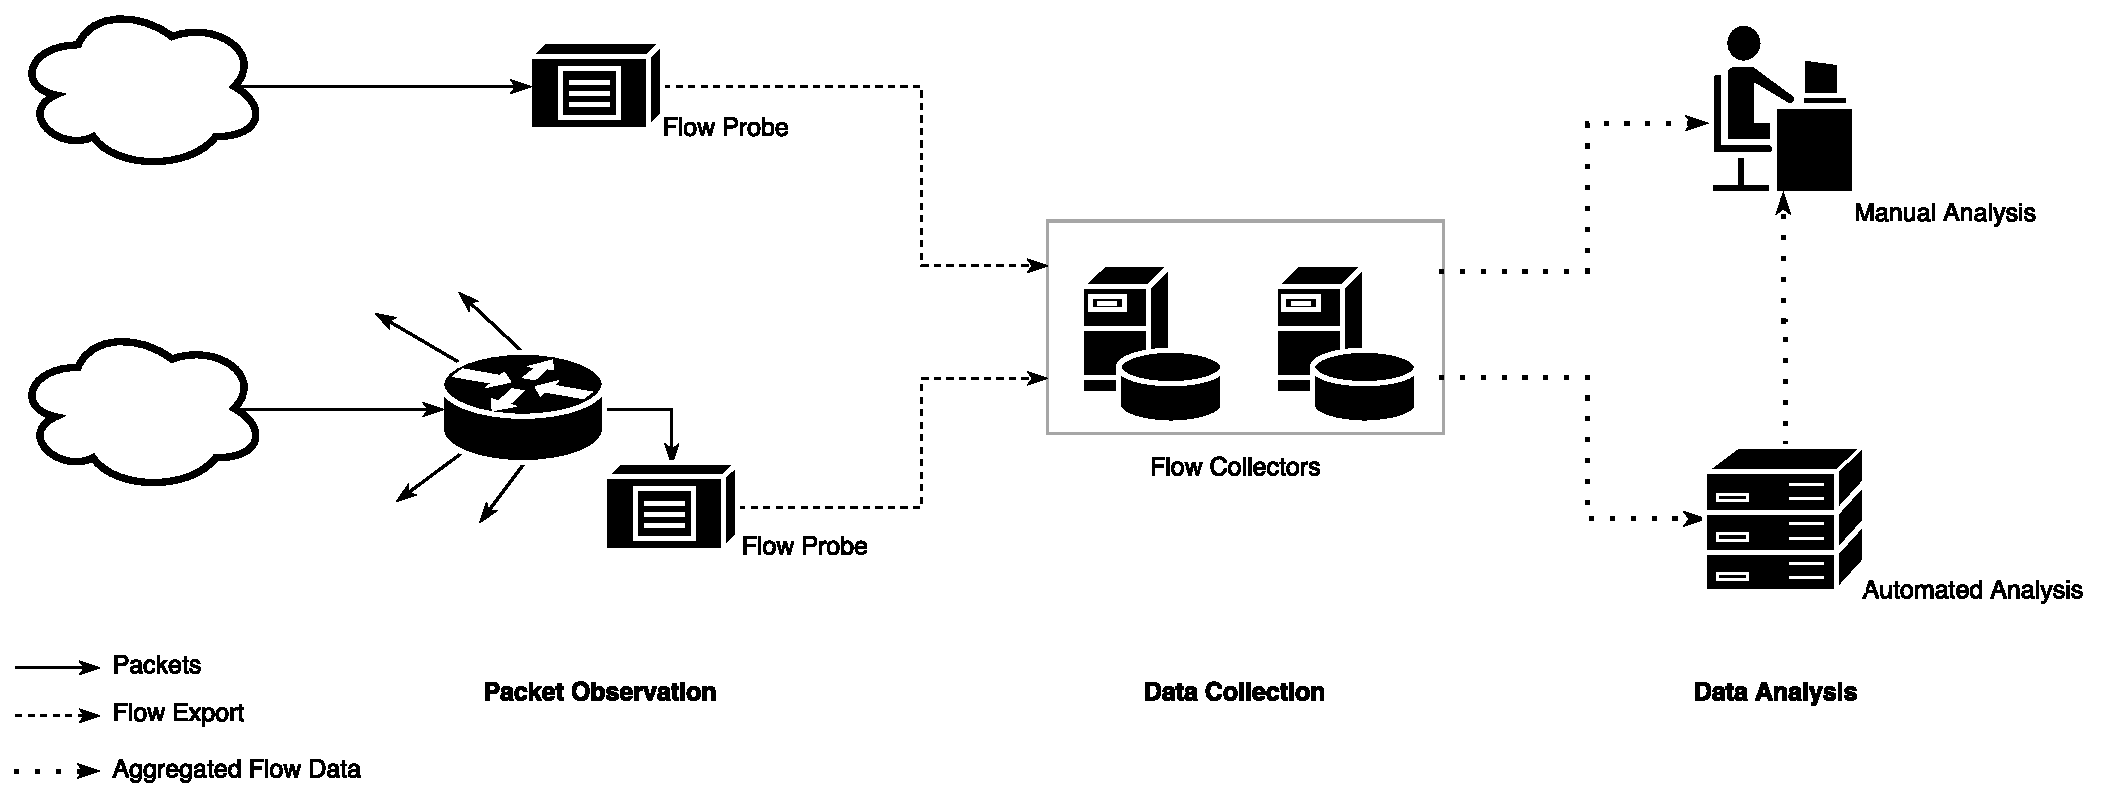
\includegraphics[width=\textwidth]{figures/200-netflow-architecture.pdf}
	\caption[Simplified flow monitoring system architecture]{Simplified flow monitoring system architecture. \parencite[cf.][]{Hofstede2014} \todo{adjust font size}}
	\label{fig:background:network:netflow:architecture}
\end{figure}

Typical flow monitoring architectures can be roughly separated into 3 stages. (cf. Figure~\ref{fig:background:network:netflow:architecture})
The first one, being Packet Observation and Flow Export, will observe bypassing traffic. Further the observed traffic is aggregated into flows, using common properties as selectors. (cf. above\alert{???}) After a flow is terminated, either by closing the underlying connection or by timeout, a record of it is exported and send of to the Flow Collector.
This stage could be implemented by a stand-alone device or within an appliance like a router with flow export capability. \parencite[cf.][]{Hofstede2014}

The exported flow are then receive by the Data Collector, which main task are storage and processing.
Exported flows contain \enquote{information about a specific flow that was observed at an observation point} \parencite{Claise2013}, which may include characteristic properties like \gls{ip} addresses and port number, as well as measured properties like packet count or overall flow size in bytes. \parencite[cf.][]{Hofstede2014}
In scope of \glspl{bas}, like \gls{knx}, characteristic properties could include source and destination address, and \gls{apci}. Hop count, payload length, and \gls{tpci} would then be used as measured properties.

Finally the last stage is concerned with the data analysis. This can be done in a manual, exploratory way, which is often the case in research projects. In more production oriented setups the analysis is often automated and integrated into the Data Collector.
The data analysis commonly includes functions like traffic profiling, correlation, anomaly and intrusion detection (cf. Section~\ref{sec:background:network:ids}), and classification and characterisation. \parencite[cf.][]{Hofstede2014}
In this work mainly anomaly and intrusion detection is of interest.

% ------------------------------------------------------------------------------
\section{Anomaly, Outlier, and Novelty Detection}
\label{sec:background:network:novelty}

The analysis of flows or general network traffic as describes in Section~\ref{sec:background:network:ids:anomaly}~and referenced in Section~\ref{sec:background:network:netflow}, relies on algorithm and techniques to detect data points which deviate from the normal expected behaviour. These algorithms and techniques can be found \alert{(better phrasing)} under the term Anomaly, Outlier, or Novelty Detection.
The aim of this section is to provide a classification of these algorithms with benefits and drawbacks.
Further, an overview of the working principle is provided for a small selection of them.

% ------------------------------------------------------------------------------
\subsection[Classification of Anomaly, Outlier, and Novelty Detection]{Classification of Anomaly, Outlier, and Novelty Detection Approaches}
\label{sec:background:network:novelty:class}

\begin{comment}
	\begin{itemize}
		\item cf. \textcite{Hodge2004}
		\item Type 1: "Determine the outliers with no prior knowledge of the data" \parencite{Hodge2004}
			\subitem "unsupervised clustering" \parencite{Hodge2004}
			\subitem "assumes that errors or faults are separated from the ‘normal’ data and will thus appear as outliers" \parencite{Hodge2004}
			\subitem " predominantly retrospective and is analogous to a batch-processing system" \parencite{Hodge2004} - Requires a bunch of data to begin with
			\subitem " requires that all data be available before processing" \parencite{Hodge2004}
			\subitem "data is static" \parencite{Hodge2004}
			\subitem "two sub-techniques" \parencite{Hodge2004}
			\subitem -> "outlier diagnostic approach highlights the potential outlying points" \parencite{Hodge2004} and "prune the outliers and fit their system model to the remaining data until no more outliers are detected" \parencite{Hodge2004}
			\subitem -> "accommodation that incorporates the outliers into the distribution model generated and employs a robust classification method" \parencite{Hodge2004} which "can withstand outliers in the data and generally induce a boundary of normality around the majority of the data" \parencite{Hodge2004}
			\subitem "Non-robust methods are best suited when there are only a few outliers in the data set" \parencite{Hodge2004}
			\subitem "a robust method must be used if there are a large number of outliers to prevent this distortion" \parencite{Hodge2004}
		\item Type 2: "Model both normality and abnormality." \parencite{Hodge2004}
			\subitem "supervised classification" \parencite{Hodge2004}
			\subitem "requires pre-labelled data" \parencite{Hodge2004}
			\subitem "The entire area outside the normal class represents the outlier class" \parencite{Hodge2004}
			\subitem "best suited to static data" \parencite{Hodge2004} "classification needs to be rebuilt from first principles if the data distribution shifts" \parencite{Hodge2004}
			\subitem "can be used for on-line classification" \parencite{Hodge2004} learning while new samples are classified
			\subitem "require a good spread of both normal and abnormal data" \parencite{Hodge2004}
			\subitem "classification is limited to a ‘known’ distribution" \parencite{Hodge2004}
			\subitem "cannot always handle outliers from unexpected regions" \parencite{Hodge2004}
		\item Type 3: "Model only normality [...]" \parencite{Hodge2004}
			\subitem "novelty detection" \parencite{Hodge2004} " semi-supervised recognition or detection task" \parencite{Hodge2004}
			\subitem "needs pre-classified data but only learns data marked normal" \parencite{Hodge2004}
			\subitem "suitable for static or dynamic data" \parencite{Hodge2004}
			\subitem "can learn the model incrementally as new data arrives" \parencite{Hodge2004}
			\subitem "aims to define a boundary of normality" \parencite{Hodge2004}
			\subitem "requires the full gamut of normality to be available for training to permit generalisation" \parencite{Hodge2004} but "requires no abnormal data" \parencite{Hodge2004}
			\subitem this is good, because "Abnormal data is often difficult to obtain or expensive in many fault detection domains [...]" \parencite{Hodge2004}
			\subitem "as long as the new fraud lies outside the boundary of normality then the system will be correctly detect the fraud" \parencite{Hodge2004}
	\end{itemize}
\end{comment}

Anomaly, Outlier, or Novelty Detection describes a class of algorithms to detect data points which deviate from the expected normal behaviour.
Or as defined by \textcite{Grubbs1969}, \enquote{an outlying observation, or outlier, is one that appears to deviate markedly from other members of the sample in which it occurs.}
In the following this definition will be used as an understanding for outliers, which is exchangeable for anomaly or novelty. \alert{(think about this!)}

The general class of algorithms for Anomaly, Outlier, and Novelty Detection can be divided into 3 sub-classes, based on which kind of data the algorithms require to be trained\alert{~and executed}.
The first sub-class describes algorithms, which are able detect outliers without prior knowledge of the data, also known as unsupervised clustering.
This means, the data points in a training set are not require to be labelled as \emph{normal} or \emph{outlier}, which is archived by relying on the assumption, that non-normal data is separated from normal data, thus appearing as outlier.
Accordingly, a substantial amount of data is required to begin with, since these kind of algorithms word \enquote{predominantly retrospective} \parencite{Hodge2004}.
Thus requiring (all) data to be available before processing and assuming it to be static.
Within this technique, 2 approaches  are used for training the model. 
The first identifies potential outliers and then continues to prune them from the original data set and fit the model to the remaining data points. This is iterated until no more outliers are detected. This non-robust method is well suited when only a few outliers are in the data set.
The second approach, however, accommodates the outliers into the distribution model and then applies a robust classification method. This is a better suited for data sets with higher numbers of outliers, since a robust classification method can withstand outliers in the data set by inducing boundaries of normality around large portions of the data. \parencite[cf.][]{Hodge2004}

The second sub-class within Outlier Detection techniques works by modelling both, normality and outliers, it is also known as supervised classification.
Therefore it requires pre-labelled data in the training phase, labelled as \emph{normal} or \emph{outlier}. Since both are used to build the model, a good spread of \emph{normal} and \emph{outlying} data is required, which also limits the classification to the known distribution of such.
As a result the whole classification model needs to be rebuild from ground up, as soon as the distribution shifts.
However, a major benefit of this method is, that it is allows for training the model while new data points are being classified, which is also known as on-line classification. \parencite[cf.][]{Hodge2004}

The third and last sub-class in Outlier Detection techniques models only normality. These techniques are often described as novelty detection or semi-supervised recognition.
It requires also pre-labelled data, but compared to the second type it only works with \emph{normal} labelled data points. Consequently the full gamut of normality is required to train an precise model. On the other hand no \emph{outlying} data points are required for training, which is highly beneficial in certain, data-sparse, scenarios, when abnormal data is difficult to obtain.
However, the training data must not contain outliers, otherwise they will be assumed to be a part of normality.
Generally the aim of this approach is to establish a tight boundary around normality and is therefore suitable for static as well as dynamic data.
If a new data point lies outside of the this boundary it is considered an \emph{outlier}, if not it is part of the \emph{normal} data.

% ------------------------------------------------------------------------------
\subsubsection{k-Nearest Neighbour}
\label{sec:background:network:novelty:knn}

\begin{comment}
	\begin{itemize}
		\item \enquote{Given a collection of data points and a query point in an m-dimensional metric space, find the data point that is closest to the query point.} \parencite{Beyer1999}
		\item \enquote{determines whether or not a point lies in a sparse region of the feature space by computing the sum of the distances to the k-nearest neighbours of the point} \parencite{Eskin2002}
		\item \enquote{[...] points in dense regions will have many points near them and will have a small k-NN score} \parencite{Eskin2002}
		\item \enquote{main problem [...] is that it is computationally expensive to compute the k-nearest neighbours of each point} \parencite{Eskin2002}
	\end{itemize}
\end{comment}

Among the techniques which can be used for clustering and hence for anomaly detection \gls{knn} is one of more established one, initially published by \textcite{Fix1951}.
The problem is described, that for any given collection of data points in an m-dimensional metric feature space, to find the k nearest data points for an arbitrary query point. \parencite{Beyer1999}
It consequently uses the proximity of data points within the feature space, allowing \gls{knn} to work with unlabelled unclean data, making it a class 1 technique according to \textcite{Hodge2004}. (cf. Section~\ref{sec:background:network:ids:anomaly})

To determine if the query point is located in an sparse area, meaning it is an outlying observation, the sum of the distance to the k-nearest neighbours is calculated.
Data points with in denser area, representing normality, will have shorter distances to their neighbours. \parencite{Eskin2002}

\subsubsection{Local Outlier Factor}
\label{sec:background:network:novelty:lof}

\begin{comment}
	\begin{itemize}
		\item Proximity-based technique
		\item seems to be a good fit cf. \textcite{Lazarevic2003}
		\item works on unclean training data
		\item good selection of vectors and distance functions is required
		\item 11\% of the first 500 telegrams in \verb|eiblog.txt| are considered outliers
		\item density based
		\item base paper \textcite{Breunig2000}
		\begin{itemize}
			\item determines for each sample in the data-set its degree of \enquote{outlier-ness} \parencite{Breunig2000}
			\item definition outlier: \enquote{An outlier is an observation that deviates so much from other observations as to arouse suspicion that it was generated by a different mechanism.} \parencite{Hawkins1980}
			\item local approach
			\subitem therefore better than k-NN, because it accounts for different density of different cluster
			\subitem \enquote{most existing work in outlier detection lies in the field of statistics} \parencite{Breunig2000}
			\subitem counteracts different density of clusters \parencite{Breunig2000}
			\subitem outlier = point is further away from its nearest points than the other points are away from each other \parencite{Breunig2000}
		\end{itemize}
	\end{itemize}
\end{comment}

\begin{wrapfigure}{r}{0.5\textwidth}
	\centering
	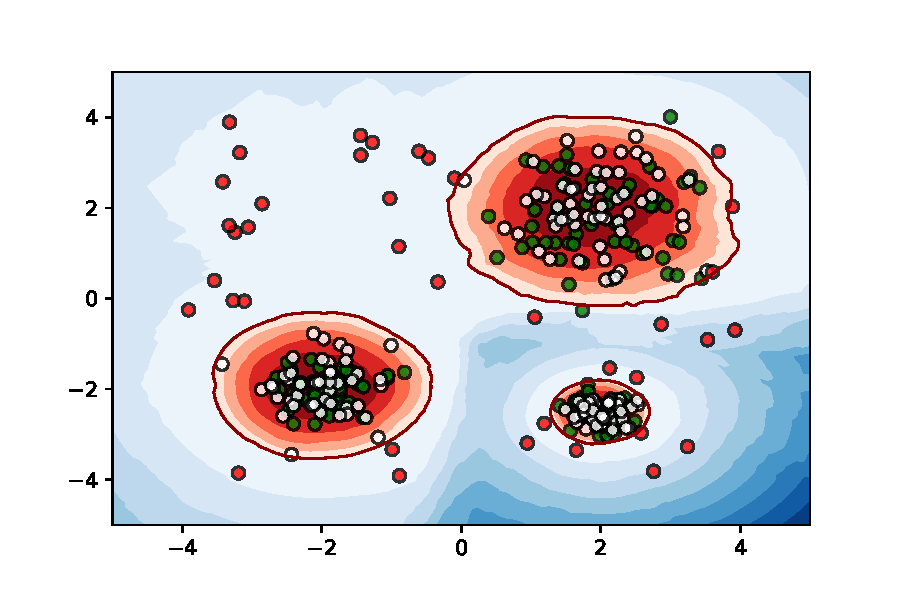
\includegraphics[width=0.48\textwidth,trim={12mm 5mm 15mm 10mm},keepaspectratio,clip]{figures/200-background-lof.pdf}
	\caption[Visualisation of the Local Outlier Factor]{Visualisation of the \gls{lof} in a 2 dimensional vector space. \emph{Green}: trainings data, \emph{Red}: outlier from test data, \emph{White}: inlier from test data. Background indicates the calculated \emph{LOF} value.}
	\label{fig:background:network:novelty:lof}
\end{wrapfigure}

Another proximity based approach to outlier detection is the \glsfirst{lof}, introduced by \textcite{Breunig2000}. It is based on the \gls{knn} problem, but accounts for locality and is specifically designed for outlier detection.
With \gls{lof} an outlier is a data point which \emph{MinPts} nearest neighbours are further away then these neighbours from each other. 
Using this lemma, For each data point the degree of \enquote{outlier-ness}, or local outlier factor, is determined.

By not relying on a global threshold, the \gls{lof} can account for clusters of different density. Therefore, one could argue, that the \gls{lof} is not only proximity based, but rather density based. Further by not treating the classification of an outlying observation as a binary property, analysis made on top of the outlier classification can be more precise. \parencite[cf.][]{Breunig2000}

Moreover, the ability of \gls{lof} to work on unclean data and account for different density in clusters through locality, making it a good match for \gls{ids} solutions, as \textcite{Lazarevic2003} shows. Also \textcite{Zanero2004} conducted an experiment on using unsupervised learning algorithms for intrusion detection and found, that the problem of locality with \gls{knn} has to be addressed in order to be more precise in predictions, what \gls{lof} archives.

\todo{ref to fig}

\subsubsection{Support Vector Machines}
\label{sec:background:network:novelty:svm}

\begin{comment}
	\begin{itemize}
		\item \enquote{The task of classification is to find a rule, which, based on external observations, assigns an object to one of several classes} \parencite{Muller2001}
		\item separate vector space by decision surfaces, setting boundaries between categories \parencite{Muller2001}
		\item \enquote{a learning algorithm for problems which are separable by hyperplanes} \parencite{Scholkopf2001a}
		\item \enquote{among all hyperplanes separating the data, there exists a unique optimal hyperplane, distinguished by the maximum margin of separation between any training point and the hyperplane} \parencite{Scholkopf2001a}
		
		\item One Class SVM
			\begin{itemize}
				\item aka. novelty detection
				\item all training data is considered good
				\item decision surface is fitted as close as possible to the training data
				\item new data outside this area, surrounded by decision surfaces, is considered an outlier
				\item \enquote{[...] does not require training data to be labelled to determine a decision surface.} \parencite{Lazarevic2003} (seems to be not exactly One-Class SVM)
				\item 
			\end{itemize}
	\end{itemize}
\end{comment}

\begin{wrapfigure}{l}{0.5\textwidth}
	\centering
	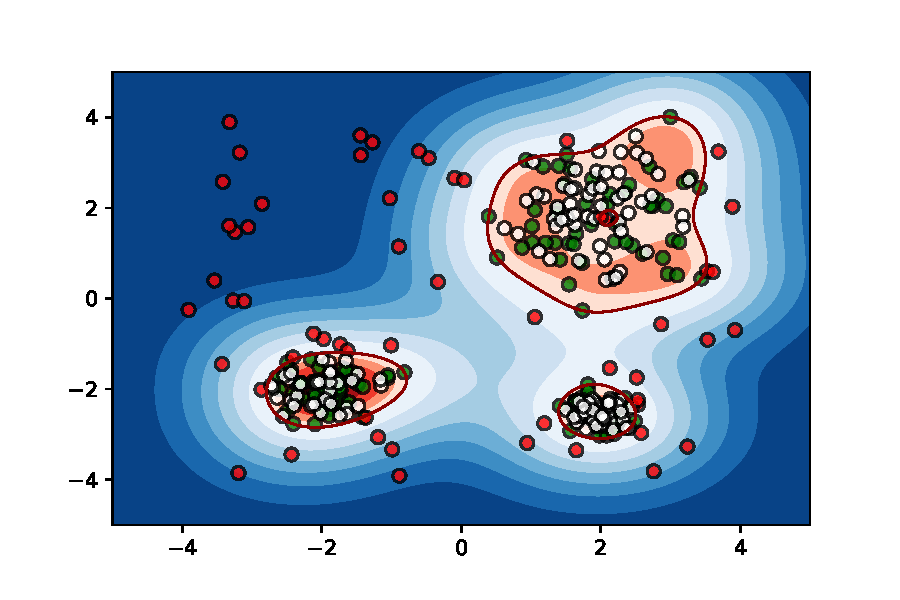
\includegraphics[width=0.48\textwidth,trim={12mm 5mm 15mm 10mm},keepaspectratio,clip]{figures/200-background-oneclass.pdf}
	\caption[Visualisation of a Support Vector Machine]{Visualisation of a \gls{svm} in a 2 dimensional vector space. \emph{Green}: trainings data, \emph{Red}: outlier from test data, \emph{White}: inlier from test data. Background indicates the distance from the decision surface.}
	\label{fig:background:network:novelty:svm}
\end{wrapfigure}

Another technique to discriminate outliers from \emph{normality} is to precisely model \emph{normality}, as \textcite{Hodge2004} described as third class of outlier detection algorithms. (cf. Section~\ref{sec:background:network:novelty:class})
\glspl{svm} are a widely used technique in this field. Especially one-class \glspl{svm} are applied in outlier and intrusion detection. \parencite[cf.][]{Lazarevic2003,Eskin2002}
They classify data points by defining decision surfaces within the feature space, which separate categories. A learning algorithm fits these hyperplanes to prior labelled data, basically finding a rule to separate data points into different classes. 
In case of one-class \gls{svm}, which are predominantly used for outlier detection, there is only one category resembling \emph{normality}. Hence the training data must contain the full gamut of normal data points, without any contamination introduced by anomalies. \parencite[cf.][]{Muller2001,Scholkopf2001a}

As \textcite{Eskin2002,Lazarevic2003} showed, \gls{svm} are a good and viable techniques to be used in anomaly-based \glspl{ids}. However, since the way this model is trained requires for clean training data, it is increasingly hard to fit it into new networks and changing environments. (cf. Section~\ref{sec:background:network:ids:anomaly})

\todo{ref to fig}

\begin{comment}
\subsubsection{Isolation Forest}
\label{sec:background:network:novelty:isoforest}
	
	\begin{itemize}
		\item \enquote{explicitly isolates anomalies rather than profiles normal instances} \parencite{Liu2008}
		\item \enquote{takes advantage of two anomalies’ quantitative properties} \parencite{Liu2008}
			\subitem \enquote{they are the minority}
			\subitem \enquote{have attribute-values that are very different}
	\end{itemize}
\end{comment}

\subsubsection{Entropy-based Outlier Detection}
\label{sec:background:network:novelty:entropy}

The information entropy, introduced by \textcite{Shannon1948}, provides an effective way to determine the uncertainty of a given system or the information content of a variable. It is further also referred to as measurement for randomness. Especially later one is intuitively related to outlier detection.

\textcite{Toshniwal2014} are using these characteristics and propose an algorithm to cluster data streams and determine outliers. 
The basic principle is to try to fit every occurring data point to every existing cluster. The data point is then finally assigned to the cluster, where it produces the least increase of entropy. Finally, the relative change of entropy for assigning a data point to the nearest cluster (\emph{PCE}) is calculated. If this \emph{PCE} is higher than a prior defined threshold, the data point is considered an outlier.
However, this method requires access to all previous data points, which implies a high resource utilisation. To increase performance \textcite{Toshniwal2014} are only keeping a window of data in memory.
Further, it might be to consider to determine a kernel function, fitted to the individual dimensions. The entropy could then be calculated against the distribution function, rather than raw data.

\begin{comment}
\subsection{Elliptical Envelope}
\label{sec:background:network:novelty:envelope}
	
	\begin{itemize}
		\item tries to fit data to estimated \emph{shape}
		\item does not seem to be a good match, since it required to know the distribution of the vector fields
	\end{itemize}

\subsection{Statistical techniques}
\label{sec:background:network:novelty:stat}

\begin{itemize}
	\item "Some [...] are applicable only for single dimensional data sets" \parencite{Hodge2004}
	\item "requires no user parameters as all parameters are derived directly from data" \parencite{Hodge2004}
	\item e.g. "Grubbs’ method (extreme studentized deviate) (Grubbs, 1969) which calculates a Z value as the difference between the mean value for the attribute and the query value divided by the standard deviation for the attribute where the mean and standard deviation are calculated from all attribute values including the query value. The Z value for the query is compared with a 1\% or 5\% significance level" \parencite{Hodge2004} also cf. \textcite{Grubbs1969}
\end{itemize}

\subsection{Proximity-based techniques}
\label{sec:background:network:novelty:prox}

\begin{itemize}
	\item "no prior assumptions about the data distribution" \parencite{Hodge2004}
	\item "not feasible for high dimensionality data sets" \parencite{Hodge2004}
\end{itemize}	


%\subsection{Bayesian}
%\subsection{Pattern Matching}
\subsection{Autoassociative Kernel Regression (AAKR)}
	used by \textcite{Yang2006}
\end{comment}

%\section{Time-based Anomaly Detection}

\subsection{Methods of Feature Encoding}
\label{sec:background:network:features}

Most algorithms and techniques for Outlier Detection (cf. Section~\ref{sec:background:network:novelty}) work within a multi-dimensional vector space or feature space. Often it is not straight forward to map specific features of a data set into a vector space.
Problematic cases included when the possible expressions of a feature need to be model as equidistant to each other.
Alternatively, in certain cases it is necessary to reduce the amount of dimension a feature would add, because otherwise the resource utilisation would exceed sane boundaries.

\subsubsection{One-Hot Encoding}
\label{sec:background:network:features:onehot}

Certain features in a dataset can represent markers or flags. In traditional data processing flags are often encoded as bit-field, where each bit represents one specific flag or marker, or as numerical value, where each number represents a state.
When using machine learning techniques, like Outlier Detection, directly on bit-fields or numerical encoded flags, a problem arises, especially with proximity base approaches.

For instance the \gls{apci} value encodes the application type in a \gls{knx} telegram as numerical value. (cf. Section~\ref{sec:background:bas:knx:communication})
For instance a \code{A\_GROUP\_VALUE\_WRITE} telegram is encoded with a value of \code{128}, whereby an \code{A\_GROUP\_VALUE\_READ} is encoded with a value of \code{000}, and \code{A\_INDIVIDUAL\_ADDRESS\_WRITE} with \code{192}.
The euclidean distance between those different \gls{apci} values would be 128, 64, and 0, which would indicate some kind of hierarchy or order.

However, for the sake of determining outliers, it is only of relevance if these values differ, the possibly induced hierarchy or order does not provide any information.
In other words the different expressions of this feature must be kept equidistant to each other.

To archive this, it is suggested in literature, to encode each expression as own dimension and only setting the expressed one to 1, leaving the rest at 0. This is referred to as \emph{one-hot} encoding. \parencite[cf.][]{Coates2011}

\subsubsection{Feature Hashing}
\label{sec:background:network:features:hashing}

When introducing multiple features in the vector space, the  amount of dimensions can increase rapidly, especially when using techniques like one-hot encoding (cf. Section~\ref{sec:background:network:features:onehot}).
This has huge implications with regards to resource consumption and more importantly to the feasibility of used algorithms on the vector space.
For instance proximity based approaches to Outlier Detection do not perform well in high dimensional vector spaces. \alert{cite needed}

To reduce the number of dimensions the amount of features could be reduced, or one could compress the feature vector. One method to archive compression by maintaining the informative value is called Feature Hashing or Kernel Trick. \parencite{Weinberger2009,Shi2009}
As the name suggests a specialised hash function is applied to the feature value to reduce the required dimensions down to a defined size.
This process is non reversible, which might have implications for further processing the results, e.g. using the coordinates of decision planes in \glspl{svm}.
Further, feature hashing introduces the possibility of hash collisions, especially when the targeted dimension number is low. Therefore the reduction needs to be considered carefully.
However, when compared to a random projection, to reduce dimensionality, the hashing-trick preserves the density and introduces no additional overhead. \parencite{Weinberger2009,Shi2009}

\subsubsection{Encoding Time}
\label{sec:background:network:features:time}

Encoding time in machine learning and in the context of anomaly detection has to be considered carefully.
First, time can not be simply expressed as \gls{unixts}, since it is not recurring by design, therefore providing no point to correlate future data points to.
As a consequence. time has to be within a seasonal context. This can be a week, a year, or any other season time range, in which events reoccur.
For example, human behaviour tends to organised in a weekly rhythm. This would make a week our reoccurring cycle. Within this cycle one could express time as seconds since the beginning of the week, e.g. Monday 00:00, and normalised against the length of a week in seconds.

Another approach on how to incorporate time could be to train several models, each one representing a fraction of the seasonal cycle. For instance, the week could be divided by days, and there would a model for Monday, a model for Tuesday, etc. pp.
However, doing this might introduce problems at the transition points between those models. So might an action which in the training set never occurred on a Monday, but always on Tuesdays only a few minutes past midnight, be considered an outlier simply due to the fact that it never happen to be trained in the Monday model.
The overall consequence is, that a few minutes in timing can change the decision surface dramatically, which is used to determine the \emph{normality.}

To mitigate these drawbacks, one could train the double amount of models, but with half of them shifted by half a time step. This would result in 14 models in our example. The first half would be normal day models, reaching from midnight to midnight. The second half, however, would be shifted by 12 hours and therefore reaching from noon to noon.

\todo{include fig from concept}

\begin{comment}
\begin{itemize}
	\item use feature direct as vector-dimension (not so good)
	\item OneHot encoding
		\subitem one vector-dimension per possible feature vector
		\subitem if feature has specific value, set dimension for this value to 1, the rest 0
		\subitem also cf. \textcite[][p. 12]{Eskin2002}, not mentioned as term, but good math-like description
		\subitem reversible
	\item Feature Hashing / Hashing Trick
		\subitem defined amount of dimensions
		\subitem feature value is hashed
		\subitem hash value is then used
		\subitem non reversible
		\subitem possibility of hash collision
		\subitem esp. when dimension count is low
		\subitem \enquote{\emph{hashing-trick:} one hashes high dimensional input vectors $x$ into a \emph{lower} dimensional feature space $\mathbb{R}^m$ with $\phi: X \rightarrow \mathbb{R}^m$} \parencite{Weinberger2009,Shi2009,Langford2007}
		\subitem \enquote{Different from random projections, the hashing-trick preserves sparsity and introduces no additional overhead to store projection matrices} \parencite{Weinberger2009}
	\item "normalize all [...] attributes to the number of standard deviations away from the mean." \parencite{Eskin2002}
		\subitem "scale based on the likelihood of the attribute values" \parencite{Eskin2002}
\end{itemize}
\end{comment}
	
	\chapter{Conceptual Architecture}
	% concept
	\label{sec:concept}
	% !TeX spellcheck = en_US

\section{Design of Netflow Agent}
	\subsection{Truncating and Statistic Gathering}

\section{Monitor Pipeline}

\section{Anomaly detection}

	\subsection{Anomaly Detection Methods}
	
	\subsubsection{Approaches}
		\begin{itemize}
			\item cf. \textcite{Hodge2004}
			\item Type 1: "Determine the outliers with no prior knowledge of the data" \parencite{Hodge2004}
				\subitem "unsupervised clustering" \parencite{Hodge2004}
				\subitem "assumes that errors or faults are separated from the ‘normal’ data and will thus appear as outliers" \parencite{Hodge2004}
				\subitem " predominantly retrospective and is analogous to a batch-processing system" \parencite{Hodge2004} - Requires a bunch of data to begin with
				\subitem " requires that all data be available before processing" \parencite{Hodge2004}
				\subitem "data is static" \parencite{Hodge2004}
				\subitem "two sub-techniques" \parencite{Hodge2004}
				\subitem -> "outlier diagnostic approach highlights the potential outlying points" \parencite{Hodge2004} and "prune the outliers and fit their system model to the remaining data until no more outliers are detected" \parencite{Hodge2004}
				\subitem -> "accommodation that incorporates the outliers into the distribution model generated and employs a robust classification method" \parencite{Hodge2004} which "can withstand outliers in the data and generally induce a boundary of normality around the majority of the data" \parencite{Hodge2004}
				\subitem "Non-robust methods are best suited when there are only a few outliers in the data set" \parencite{Hodge2004}
				\subitem "a robust method must be used if there are a large number of outliers to prevent this distortion" \parencite{Hodge2004}
			\item Type 2: "Model both normality and abnormality." \parencite{Hodge2004}
				\subitem "supervised classification" \parencite{Hodge2004}
				\subitem "requires pre-labelled data" \parencite{Hodge2004}
				\subitem "The entire area outside the normal class represents the outlier class" \parencite{Hodge2004}
				\subitem "best suited to static data" \parencite{Hodge2004} "classification needs to be rebuilt from first principles if the data distribution shifts" \parencite{Hodge2004}
				\subitem "can be used for on-line classification" \parencite{Hodge2004} learning while new samples are classified
				\subitem "require a good spread of both normal and abnormal data" \parencite{Hodge2004}
				\subitem "classification is limited to a ‘known’ distribution" \parencite{Hodge2004}
				\subitem "cannot always handle outliers from unexpected regions" \parencite{Hodge2004}
			\item Type 3: "Model only normality [...]" \parencite{Hodge2004}
				\subitem "novelty detection" \parencite{Hodge2004} " semi-supervised recognition or detection task" \parencite{Hodge2004}
				\subitem "needs pre-classified data but only learns data marked normal" \parencite{Hodge2004}
				\subitem "suitable for static or dynamic data" \parencite{Hodge2004}
				\subitem "can learn the model incrementally as new data arrives" \parencite{Hodge2004}
				\subitem "aims to define a boundary of normality" \parencite{Hodge2004}
				\subitem "requires the full gamut of normality to be available for training to permit generalisation" \parencite{Hodge2004} but "requires no abnormal data" \parencite{Hodge2004}
				\subitem this is good, because "Abnormal data is often difficult to obtain or expensive in many fault detection domains [...]" \parencite{Hodge2004}
				\subitem "as long as the new fraud lies outside the boundary of normality then the system will be correctly detect the fraud" \parencite{Hodge2004}
				
		\end{itemize}
	
	\subsubsection{Local Outlier Factor}
		\begin{itemize}
			\item seems to be a good fit
			\item works on unclean training data
			\item good selection of vectors and distance functions is required
			\item 11\% of the first 500 telegrams in \verb|eiblog.txt| are considered outliers
			\item density based
		\end{itemize}
	
	\subsubsection{On Class SVM}
		\begin{itemize}
			\item aka. novelty detection
			\item all training data is considered good
		\end{itemize}
	
	\subsubsection{Isolation Forest}
		\begin{itemize}
			\item ...
		\end{itemize}
	
	\subsubsection{Elliptical Envelope}
		\begin{itemize}
			\item tries to fit data to estimated \emph{shape}
			\item does not seem to be a good match, since it required to know the distribution of the vector fields
		\end{itemize}
	
	\chapter{Results}
	% ...
	
	\chapter{Prototype Implementation}
	
	\chapter{Discussion}
	% discussion (duh)
	
	
	% --------------------------------------------------------------------------
	% statement of own work
	\newpage
	\pagenumbering{gobble}  % turn off page numbering for this page
	
	\chapter*{Selbstständigkeitserklärung}
	Hiermit erkläre ich Martin Peters, dass ich die vorliegende Bachelorarbeit selbständig angefertigt habe. Es wurden nur die in der Arbeit ausdrücklich benannten Quellen und Hilfsmittel benutzt. Wörtlich oder sinngemäß übernommenes Gedankengut habe ich als solches kenntlich gemacht.
	\\[64pt]
	\noindent Rostock, \thedate
	\begin{flushright}
		$\overline{~~~~~~~~~\mbox{(Unterschrift)}~~~~~~~~~}$
	\end{flushright}
	
	% restart page numbering
	\newpage
	\pagenumbering{Roman}
	
	% --------------------------------------------------------------------------
	% Bibliography
	%\nocite{*}
	\printbibliography
	
	% --------------------------------------------------------------------------
	% Appendix
	\begin{appendices}
		\noappendicestocpagenum
		\addappheadtotoc
		
		%\chapter*{Appendix}
		\label{sec:appendix}
		% !TeX spellcheck = en_US
% ------------------------------------------------------------------------------
% code highlighting
% some nice styling for code listings
\definecolor{mygreen}{rgb}{0,0.6,0}
\definecolor{mygray}{rgb}{0.5,0.5,0.5}
\definecolor{mymauve}{rgb}{0.58,0,0.82}
\definecolor{lightgray}{rgb}{0.97,0.97,0.97}
%
\lstset{ %
	backgroundcolor=\color{lightgray},   % choose the background color; you must add \usepackage{color} or \usepackage{xcolor}
	basicstyle=\footnotesize,        % the size of the fonts that are used for the code
	breakatwhitespace=false,         % sets if automatic breaks should only happen at whitespace
	breaklines=true,                 % sets automatic line breaking
	captionpos=b,                    % sets the caption-position to bottom
	commentstyle=\color{mygreen},    % comment style
	deletekeywords={...},            % if you want to delete keywords from the given language
	escapeinside={\%*}{*)},          % if you want to add LaTeX within your code
	extendedchars=true,              % lets you use non-ASCII characters; for 8-bits encodings only, does not work with UTF-8
	frame=single,	                   % adds a frame around the code
	framerule=0pt,
	keepspaces=true,                 % keeps spaces in text, useful for keeping indentation of code (possibly needs columns=flexible)
	%keywordstyle=\color{blue},       % keyword style
	%keywordstyle={},
	language=Octave,                 % the language of the code
	otherkeywords={*,...},           % if you want to add more keywords to the set
	numbers=left,                    % where to put the line-numbers; possible values are (none, left, right)
	numbersep=5pt,                   % how far the line-numbers are from the code
	numberstyle=\tiny\color{mygray}, % the style that is used for the line-numbers
	rulecolor=\color{black},         % if not set, the frame-color may be changed on line-breaks within not-black text (e.g. comments (green here))
	showspaces=false,                % show spaces everywhere adding particular underscores; it overrides 'showstringspaces'
	showstringspaces=false,          % underline spaces within strings only
	showtabs=false,                  % show tabs within strings adding particular underscores
	stepnumber=2,                    % the step between two line-numbers. If it's 1, each line will be numbered
	%stringstyle=\color{mymauve},     % string literal style
	stringstyle=\textit,
	tabsize=2,	                   % sets default tabsize to 2 spaces
	title=\lstname                   % show the filename of files included with \lstinputlisting; also try caption instead of title
}
%
% ------------------------------------------------------------------------------


	\end{appendices}
\end{document}
